\begin{center}
\begingroup
\fontsize{18}{20}\selectfont {\bf UNIVERSIDAD NACIONAL}\\
\fontsize{18}{20}\selectfont {\bf \Large AGRARIA LA MOLINA}\\
\vspace{0.55cm}
\fontsize{16}{14}\selectfont {\bf \Large ESCUELA DE POSGRADO} \\
\vspace{0.25cm}
\fontsize{14}{12}\selectfont {\bf MAESTRÍA EN RECURSOS HÍDRICOS} \\
\vspace{1.85cm}

\begin{figure}[!h]
  \centering
  
\includegraphics[width=0.3\textwidth]{Images/logoUNALM.png}
\end{figure}

\vspace{0.85cm}

\fontsize{14pt}{12pt}\selectfont {\bf “VULNERABILIDAD DE LA DISPONIBILIDAD}\\
\vspace{0.25cm}
\fontsize{14pt}{12pt}\selectfont {\bf DE LOS RECURSOS HÍDRICOS EN EL PERÚ}\\
\vspace{0.25cm}
\fontsize{14pt}{12pt}\selectfont {\bf FRENTE AL CAMBIO CLIMÁTICO: ANÁLISIS}\\
\vspace{0.25cm}
\fontsize{14pt}{12pt}\selectfont {\bf PROBABILÍSTICO DE BUDYKO”}\\
\vspace{1.5cm}

\fontsize{14pt}{14pt}\selectfont {\bf Presentado por: }\\
\vspace{0.5cm}
\fontsize{14pt}{14pt}\selectfont {\bf ADRIAN MARKO HUERTA JULCA}\\
\vspace{1.5cm}

\fontsize{14pt}{14pt}\selectfont {\bf TESIS PARA OPTAR EL GRADO DE MAESTRO}\\
\vspace{0.25cm}
\fontsize{14pt}{14pt}\selectfont {\bf MAGÍSTER SCIENTIAE EN RECURSOS HÍDRICOS}\\
\vspace{1.5cm}

\fontsize{14pt}{12pt}\selectfont {\bf Lima - Perú}\\
\vspace{0.25cm}
\fontsize{14pt}{12pt}\selectfont {\bf 2020}\\

\endgroup
\end{center}
\newpage


%=====================  REGISTRO DE FIRMAS  =========================
%  \begin{center}
%  	\begingroup
% \fontsize{18}{20}\selectfont {\bf UNIVERSIDAD NACIONAL}\\
% \fontsize{18}{20}\selectfont {\bf AGRARIA LA MOLINA}\\
% \vspace{0.55cm}
% \fontsize{16}{14}\selectfont {\bf \Large ESCUELA DE POSGRADO} \\
% \vspace{0.25cm}
% \fontsize{14}{12}\selectfont {\bf MAESTRÍA EN RECURSOS HÍDRICOS} \\
% \vspace{1cm}
    
% \fontsize{14pt}{12pt}\selectfont {\bf “VULNERABILIDAD DE LA DISPONIBILIDAD}\\
% \vspace{0.25cm}
% \fontsize{14pt}{12pt}\selectfont {\bf DE LOS RECURSOS HÍDRICOS EN EL PERÚ}\\
% \vspace{0.25cm}
% \fontsize{14pt}{12pt}\selectfont {\bf FRENTE AL CAMBIO CLIMÁTICO: ANÁLISIS}\\
% \vspace{0.25cm}
% \fontsize{14pt}{12pt}\selectfont {\bf PROBABILÍSTICO DE BUDYKO”}\\

%  	\vspace{.75cm}
	
% \fontsize{14pt}{12pt}\selectfont {\bf TESIS PARA OPTAR EL GRADO DE MAESTRO}\\
% \vspace{0.25cm}
% \fontsize{14pt}{12pt}\selectfont {\bf MAGÍSTER SCIENTIAE EN RECURSOS HÍDRICOS}\\

% 	\vspace{1cm}
	
% 	\fontsize{12pt}{12pt}\selectfont {\bf Presentado por: }\\
% 	\vspace{0.5cm}
	
% 	\fontsize{14pt}{12pt}\selectfont {\bf Adrian Marko Huerta Julca}\\
	
% 	\vspace{0.5cm}
	
% 	\fontsize{12pt}{12pt}\selectfont {\bf Sustentado y aprobado ante el siguiente Jurado:}\\
	
% 	\endgroup
	
% 	\vspace{3.2cm}
	
% 	\begin{multicols}{2}
% 		\rule[0.05cm]{7cm}{0.01cm}\\
% 		\fontsize{11pt}{10pt}\selectfont {\bf Mg.Sc. Cayo Ramos Taipe}\\
% 		\fontsize{12pt}{12pt}\selectfont {\bf PRESIDENTE}\\
		
% 		\vspace{2.5cm}
		
% 		\rule[0.05cm]{7cm}{0.01cm}\\
% 		\fontsize{11pt}{10pt}\selectfont {\bf PhD. Eduardo Chavarri Velarde}\\
% 		\fontsize{12pt}{12pt}\selectfont {\bf MIEMBRO}\\				
		
% 		\vspace{2.5cm}
		
% 		\rule[0.05cm]{7cm}{0.01cm}\\
% 		\fontsize{11pt}{10pt}\selectfont {\bf Dr. Waldo Lavado Casimiro}\\
% 		\fontsize{12pt}{12pt}\selectfont {\bf PATROCINADOR}\\
		
% 		\vspace{2.5cm}
		
% 	\rule[0.05cm]{7cm}{0.01cm}\\
% 	\fontsize{11pt}{10pt}\selectfont {\bf Mg.Sc. Ricardo Apaclla Nalvarte}\\
% 	\fontsize{12pt}{12pt}\selectfont {\bf MIEMBRO}\\
% 	\end{multicols}
% 	\vspace{2.2cm}

% \rule[0.05cm]{7cm}{0.01cm}\\
% \fontsize{11pt}{10pt}\selectfont {\bf Dr. Waldo Lavado Casimiro}\\
% \fontsize{12pt}{12pt}\selectfont {\bf CO-PATROCINADOR}\\
% \end{center}
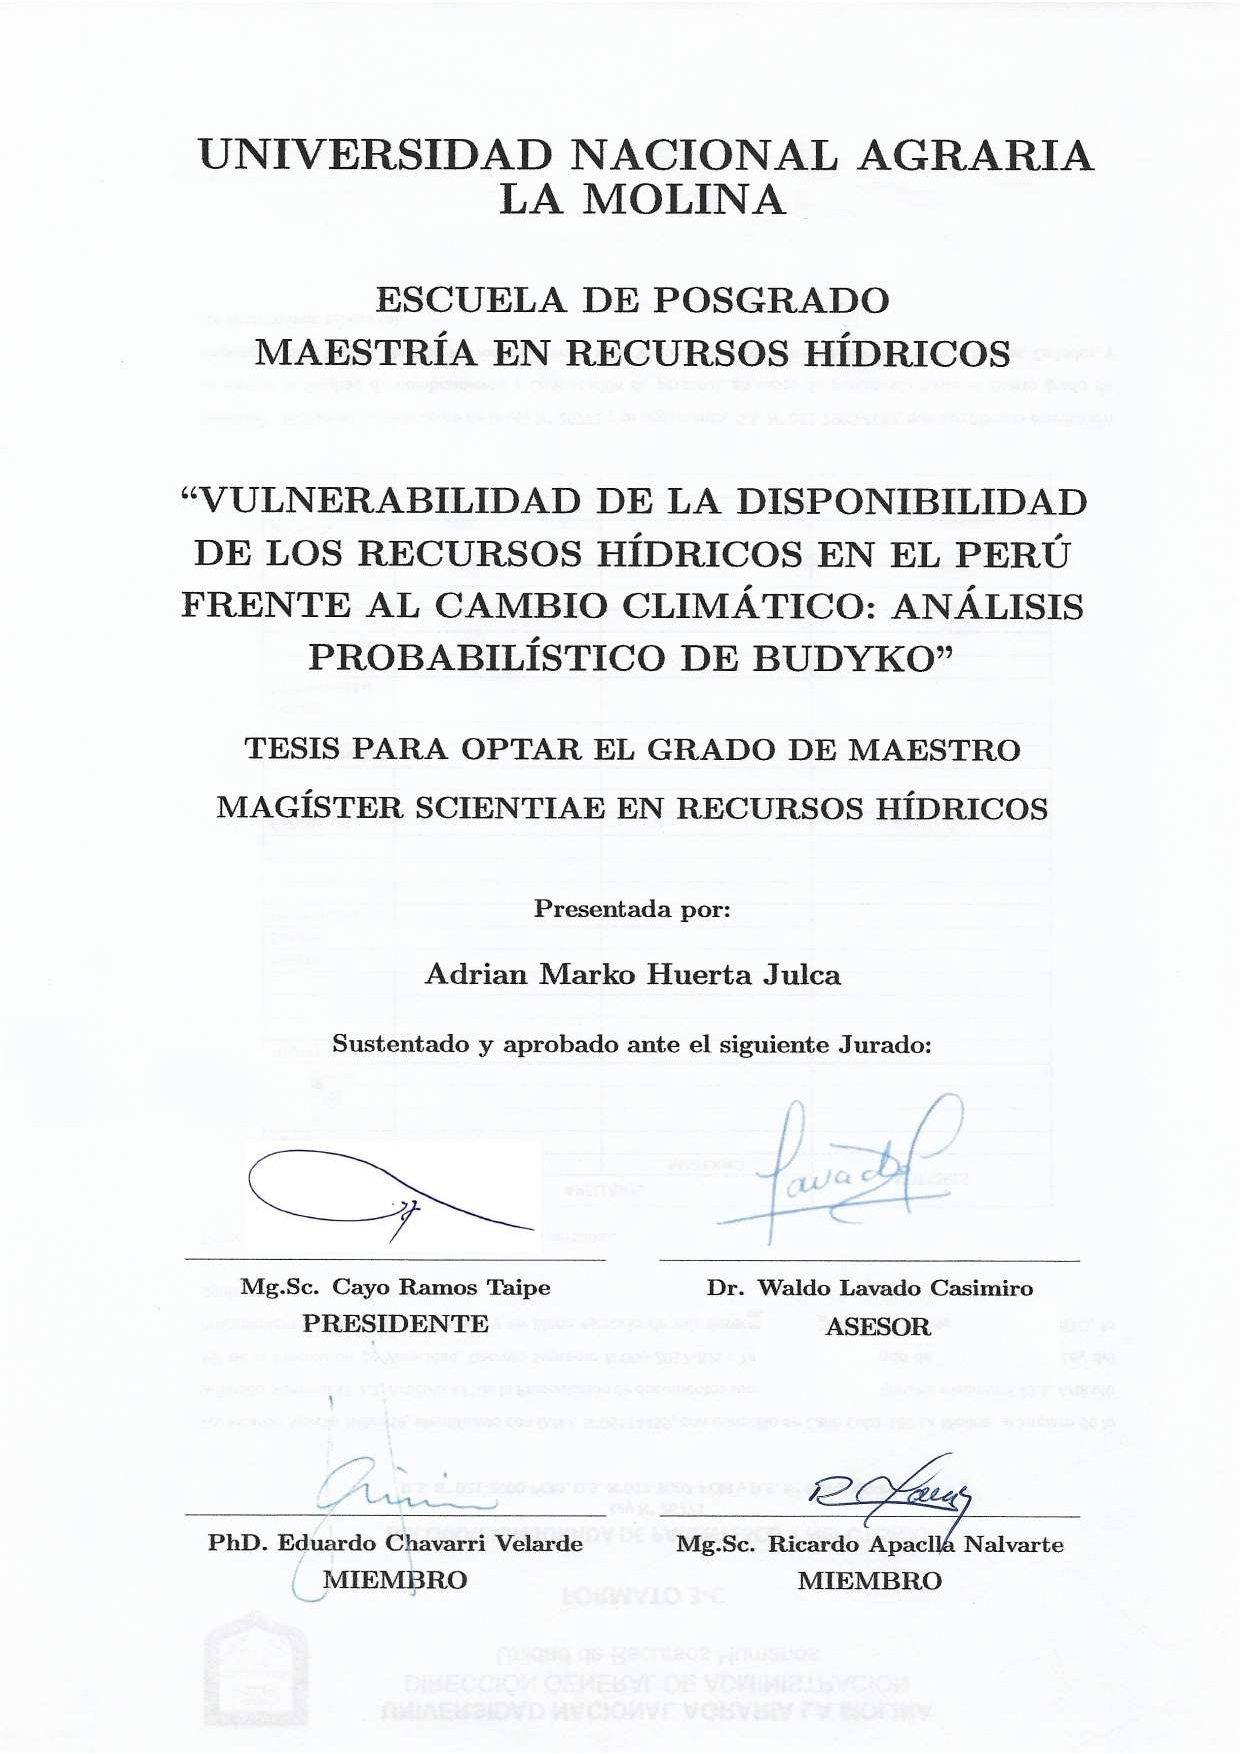
\includepdf[pages=1,fitpaper]{FigsANDTables/firma_jurado}
\clearpage
%=====================  ACTA DE SUSTENTACIÓN ====================
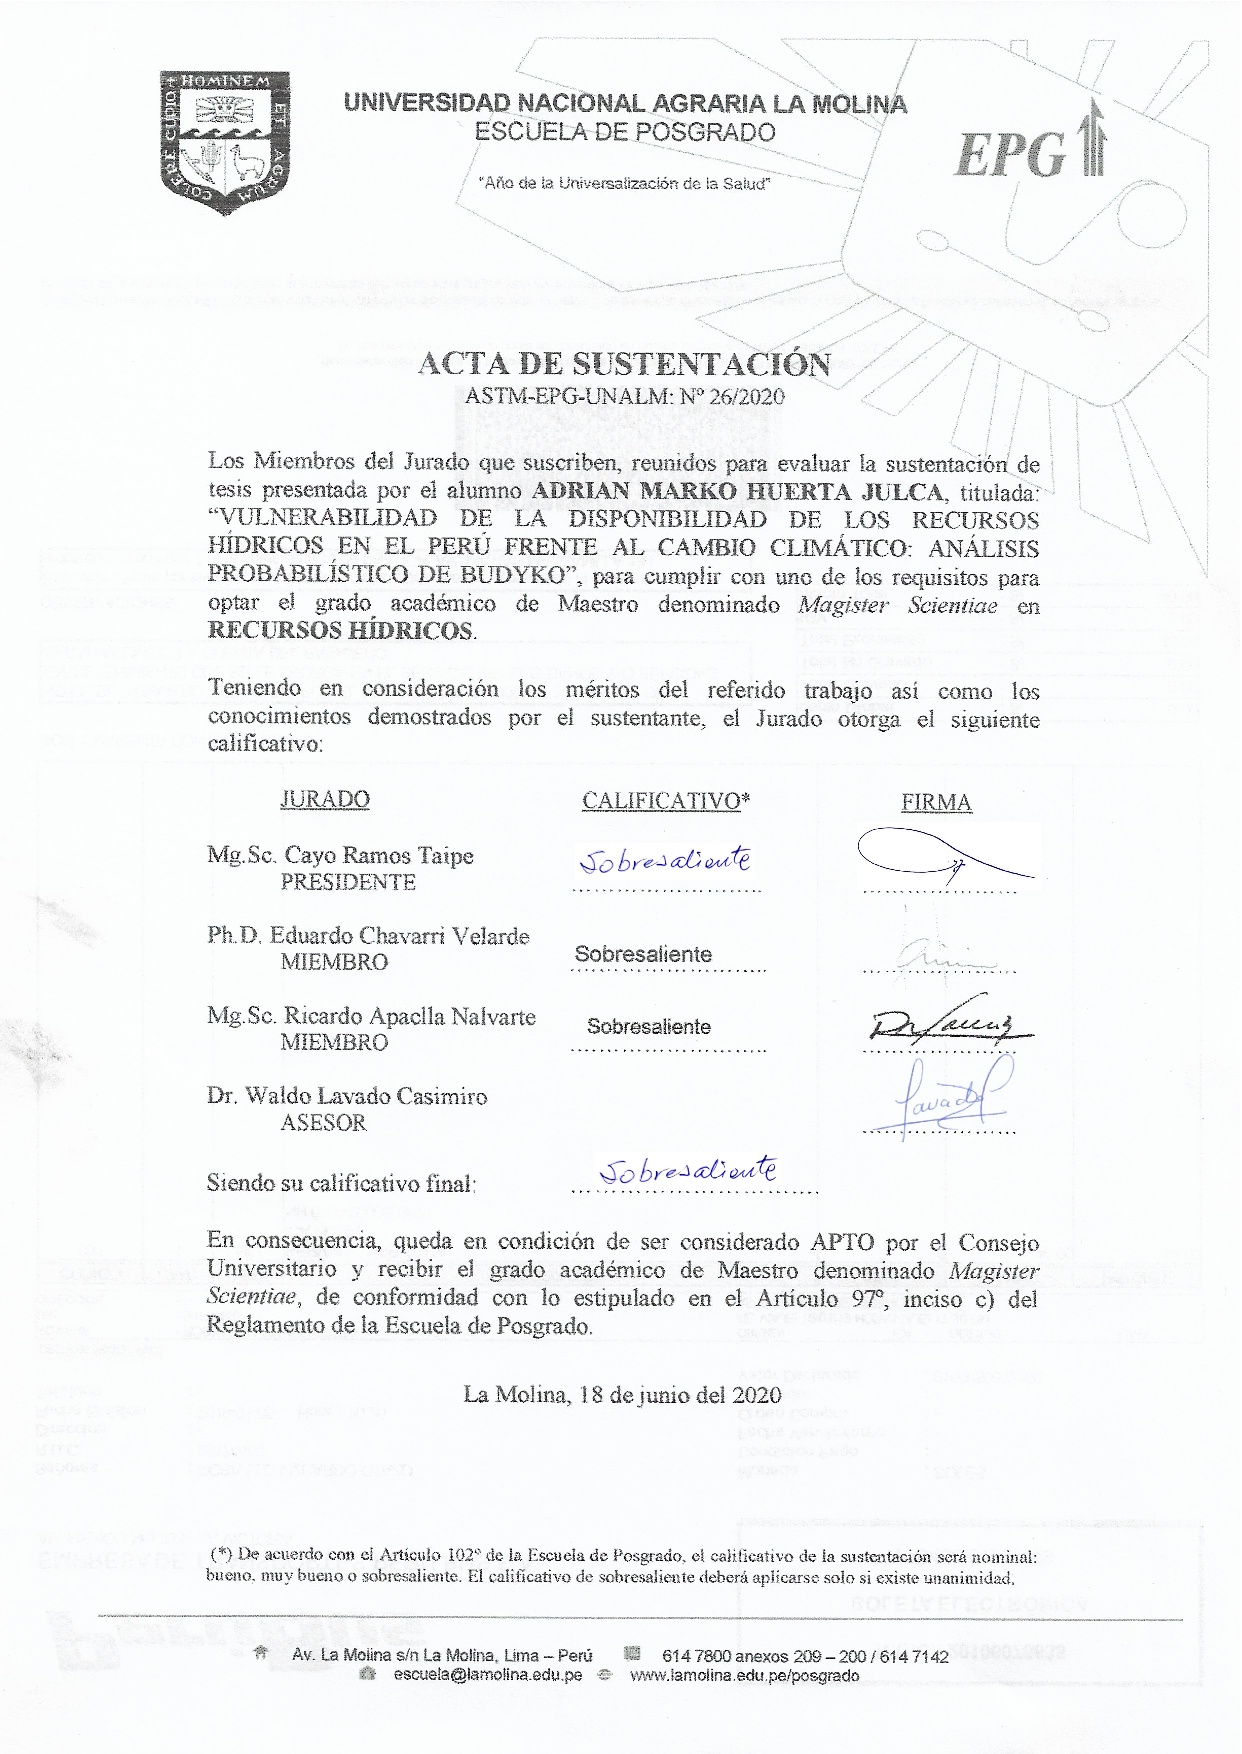
\includepdf[pages=1,fitpaper]{FigsANDTables/acta_sustentacion}
\clearpage
%=====================  DEDICATORIA  =========================
\begin{center}
\large{\textbf {DEDICATORIA}}
\end{center}

\begin{flushright}
A mi abuelo Adriano, a mis padres Jaime y \textit{Luciana}; hermanos y hermanas por su enorme apoyo, esfuerzo y comprensión durante mi segunda etapa de aprendizaje que inicio con mis estudios en la Maestría.
\end{flushright}

\clearpage
%=====================  AGRADECIMIENTOS  =========================
\begin{center}
\large{\textbf {AGRADECIMIENTOS}}
\end{center}

\begin{flushright}

La presente investigación se llevo a cabo gracias a la ejecución del Proyecto RAHU con Contrato N$^{\circ}$ 005-2019-FONDECYT “Water Security and Climate Change adaptation in Peruvian glacier-fed rivers basins”, financiado por el Fondo Newton-Paulet, a través de NERC y Fondecyt.\\
Un especial agradecimiento al Dr. Waldo Lavado, quien ha asesorado la investigación, y por las interesantes discusiones y sugerencias. De igual manera a los miembros del jurado (Mg.Sc. Cayo Ramos, PhD. Eduardo Chavarri y Mg.Sc. Ricardo Apaclla) por sus útiles e importantes comentarios.\\
Adicionalmente, a todos los compañeros y amigos de la Maestría y de la Subdirección de Estudios e Investigaciones Hidrológicas (antes Hidrología Aplicada), con quienes compartí inquietudes, conocimientos y momentos muy gratos. Finalmente, pero no por ello menos importante, a mis amigos “meteoros" por los conocimientos compartidos, las aventuras y el apoyo emocional.
\end{flushright}

